\section{Problem Specifications}

\subsection{Orbit correction}

Orbit stability is a crucial and import issue of modern generation light sources. Ambient mechanical and electrical noise cause rather large orbit distortions which have to be counteracted by an orbit feedback.

\subsubsection{Instruments of Monitoring and Correction} 

In order to correct the orbit and locate the position of the particles it is necessary some instruments. In the case of PETRA, the FOFB system uses a star like structure in the cabling, where the position data, captured by the BPMs, is sent to a central processing unit. Calculations are performed in real time and digital output streams are sent to instrumentation buildings located around the ring. These streams are received by digital power amplifiers that ultimately feed the  air coil correctors. The main instruments will be briefly discussed below \cite{klute2011petra}.

\subsubsection*{Beam Position Monitors} 

The electron beam position by a sensors called Beam Position Monitors (BPM). Each monitor is composed by four electrostatic pick-up electrodes that are installed crosswise at the beam pipe wall. The electric field produced by the beam particles induces a charge on the electrodes. The difference signals of opposite electrodes yield the beam's centre of mass for both transverse planes, respectively. It is a non-destructive diagnosis (it does not affect the beam) \cite{forck2009beam} \cite{gaupp1988beam}.

\subsubsection*{Corrector Magnets}

Around the storage ring, dipole magnets called corrector magnets are used to correct the orbit. At a certain position and in a certain direction, each dipole contributes to the correction. The most effective correction is obtained when the correctors are located as near as possible to the sources of generating the largest orbit deviations, i.e. the quadrupoles \cite{fasthori26}.

\subsubsection{Methods}

To complete

\subsection{System description}

The objective of the FOFB is to mitigate fluctuations in the beam, which occurs mainly due to ground motion transmitted to the beam through the misalignment of the magnets. To accomplish this task the control system modifies the correctors setpoints which is symbolized by $\vect{u}[k]$, where $k$ is the time index. The perturbations are introduced in the model by the vector $\vect{d}[k]$, the beam is steered back to the reference orbit $r_0$. The position of the beam is measured at each instant by means of BPMs located at different positions of the ring, the vector of the measurements is $\vect{y}[k]$. 

The data obtained by the BPMs $\vect{y}[k]$ are used by the control algorithm to calculate the setpoint of the correctors $\vect{u}[k+1]$. The change in the monitors measurements $\vect{u}[k]$ due to changes in the actuators $\vect{u}[k]$ is modeled by a transfer function $g(z)$ that represent the dynamic response of the actuators and a static part which is a simple multiplication with the orbit response matrix $\matr{R}$. The schematic of the model is shown in \ref{f:sytem_simple} and can be written in the form 
\begin{align} \label{y_discrete_time}
    \vect{y}[k] = g(z) \matr{R} \vect{x}[k] + \vect{d}[k].
\end{align}

In \ref{y_discrete_time} we assume that $g(z)$ is the same for all the actuators since the same corrector magnets are used around the ring. The disturbances and the controller setpoints act on the BPM readings via different response matrix which will be discussed bellow.

\begin{figure}	
    \centering 
    \begin{tikzpicture}[auto, node distance = 1.5 cm, >=latex']
        \tikzstyle{block} = [draw, rectangle]
        \tikzstyle{sum} = [draw, circle]
        \tikzstyle{input} = [coordinate]
        \tikzstyle{output} = [coordinate]
        \tikzstyle{->} = [-latex]

        \node [input, name=input] {};
        \node [sum, right = of input] (sum) {};
        \node [block, label = {Controller}, right = of sum] (controller) {$q(z)\matr{R}^{\dagger}$};
        \node [block, label = {System}, right = of controller] (system) {$g(z)\matr{R}$};
        \node [sum, right = of system] (sum2) {};
        \node [output, label = {$\vect{y}[k]$}, name = output, right of = sum2] {};
        \node [input, above of = sum2, node distance = 1.5 cm] (inputd) {};

        \draw [->] (input) -- node {$\vect{r_0}$} (sum);
        \draw [->] (sum) -- node {} (controller);
        \draw [->] (controller) -- node {$\vect{u}[k]$} (system);
        \draw [->] (system) -- node {} (sum2);
        \draw [->] (sum2) -- node [name=e] {} (output);
        \coordinate [below of = e, node distance = 1.5 cm] (tmp);
        \draw [->] (e) |- (tmp) -| node[pos=0.99] {\tiny $-$} 
            node [near end] {} (sum);
        \draw [->] (inputd) -- node[pos=0.99] {\tiny $+$} 
            node [near start] {$\vect{d}[k]$} (sum2);
    \end{tikzpicture}
    \caption{Schematic of the digital closed orbit feedback system.}
    \label{f:sytem_simple}
\end{figure}

\subsection{Orbit Response Matrix}

The orbit response matrix $\matr{R}$, is a linear relationship between a corrector magnet's strength (the extent to which it bends the beam) and the beam's position when measured horizontally or vertically by any “down-stream” Beam Position Monitor \cite{white1997hybrid}. Therefore, the column $\textrm{i}^{th}$ of $\matr{R}$ correspond to the BPMs measurements if the corrector $\textrm{i}^{th}$ is excited with a unit step (1 $\mu rad$), is shown in \ref{fig:bpm_unit_actuation}. Theoretically, the linear response of a single dipole perturbation is the well-known closed orbit formula \ref{e:rm_closed_orbit}:
\begin{equation} \label{e:rm_closed_orbit}
    \Delta z(s') = \frac{\sqrt{\beta(s) \beta(s')}}{2 \pi \sin(\pi \nu)} \Delta \theta \cos(|\phi(s) - \phi(s')| - \pi \nu)
\end{equation}
where $z$ denotes the horizontal or vertical position, $\beta$, $\phi$ are the beta function and beta phase, $\nu$ is the tune \cite{chiu2008conceptual}. It can be deducted that the orbit is proportional everywhere to the strength of the perturbation $\theta$ and to $\sqrt{\beta_o \beta_k}$ which is the amplitude of the beta function at the location of the perturbation.

If the process is repeated for all correctors and measured for all BPMs the spatial response matrix $\matr{R}$ is obtained. Although the matrix can be completely calculated theoretically using the accelerator model and physics, this methodology does not exactly represent the reality, for example, some misalignments of magnets or external magnetic perturbations would not be taken into account. It is a more common and accurate way to obtain it empirically directly on the actual ring \cite{klute2011petra}. 

In this thesis, to calculate the response matrix has been used a model of the PETRA III ring containing the information of each of its components and the tools of Accelerator Toolbox. By means of the function \textit{find\_orbit} \cite{Welcomet22:online} the particles are tracked through the ring simulation and the function of the closed orbit is obtained.

\begin{figure}
    \begin{center}
        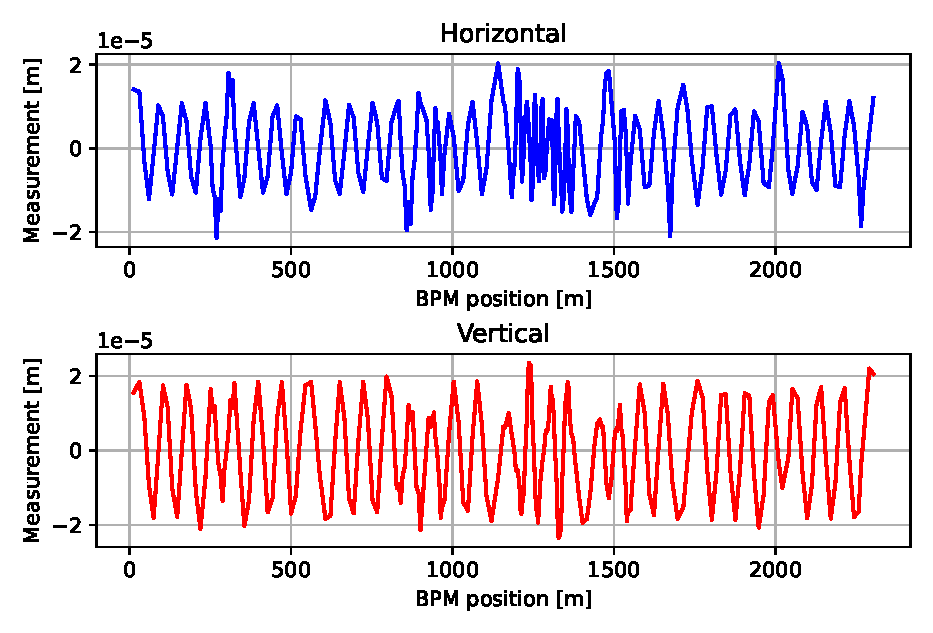
\includegraphics{bpm_unit_actuation.eps}
    \end{center}
    \caption{Readings of BPMs after applying a 1 $\mu m$ kick in the $\textrm{1}^{st}$ corrector.}
    \label{fig:bpm_unit_actuation}
\end{figure}

\begin{figure}
    \begin{center}
        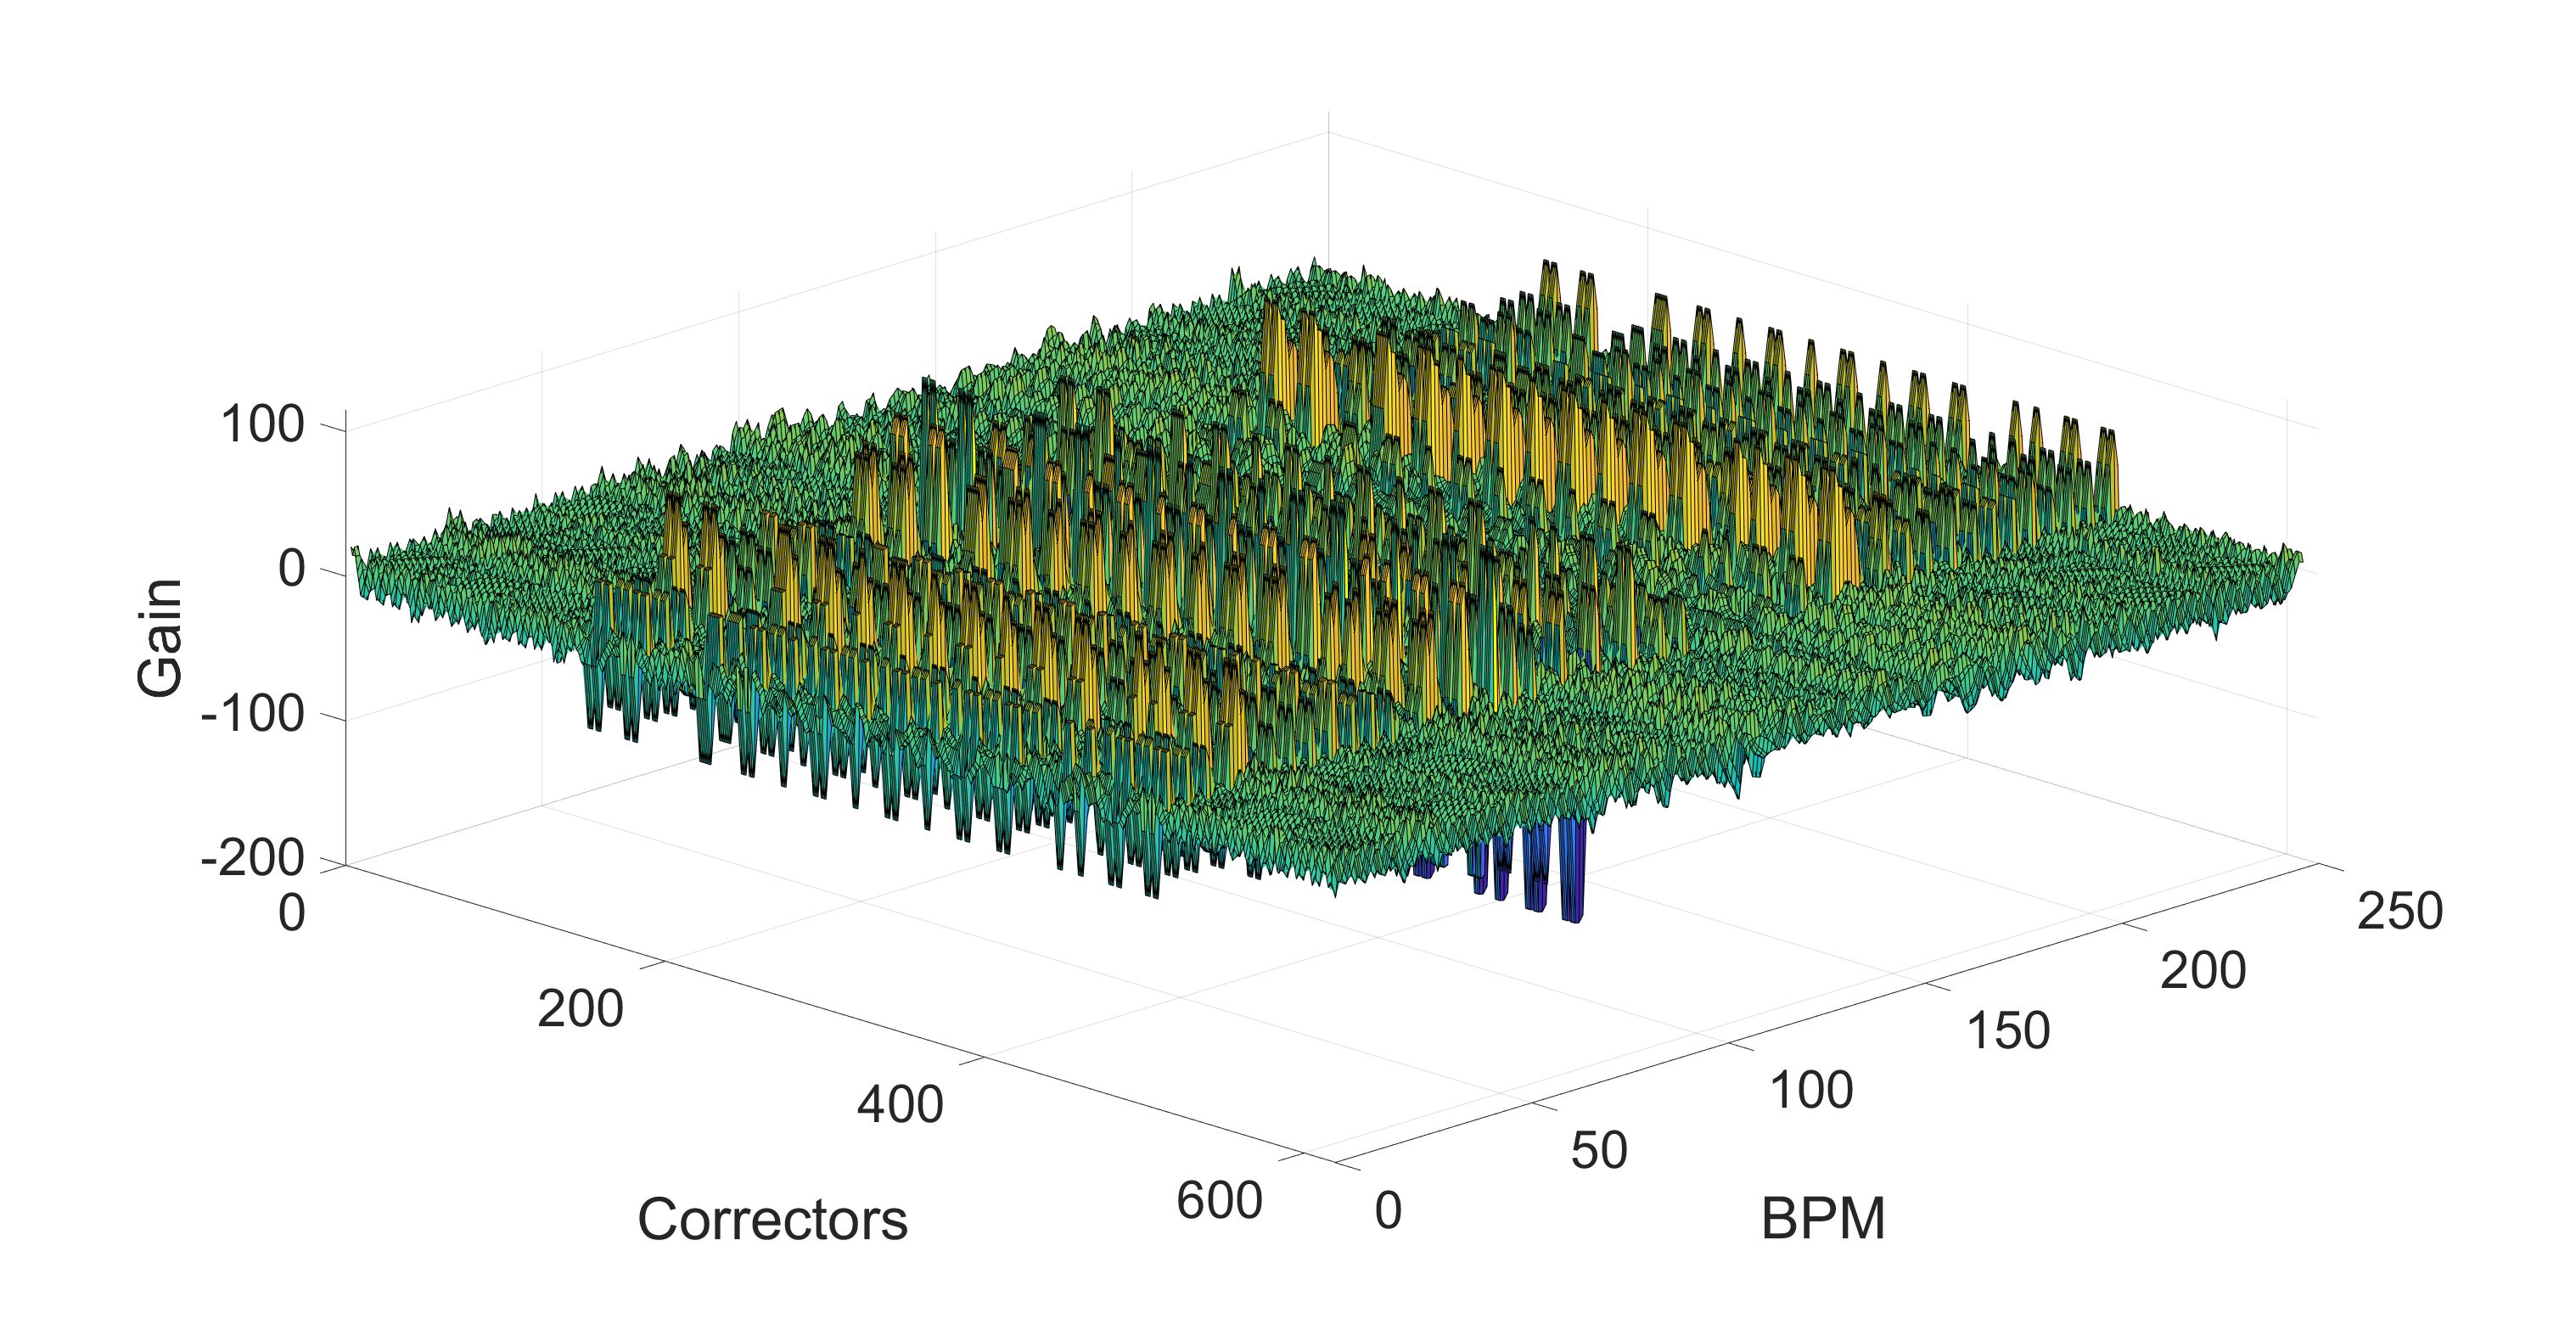
\includegraphics[scale=0.3]{R_x.eps}
    \end{center}
    \caption{Storage ring response matrix 3D plot (horizontal).}
    \label{fig:R_x}
\end{figure}

\begin{figure}
    \begin{center}
        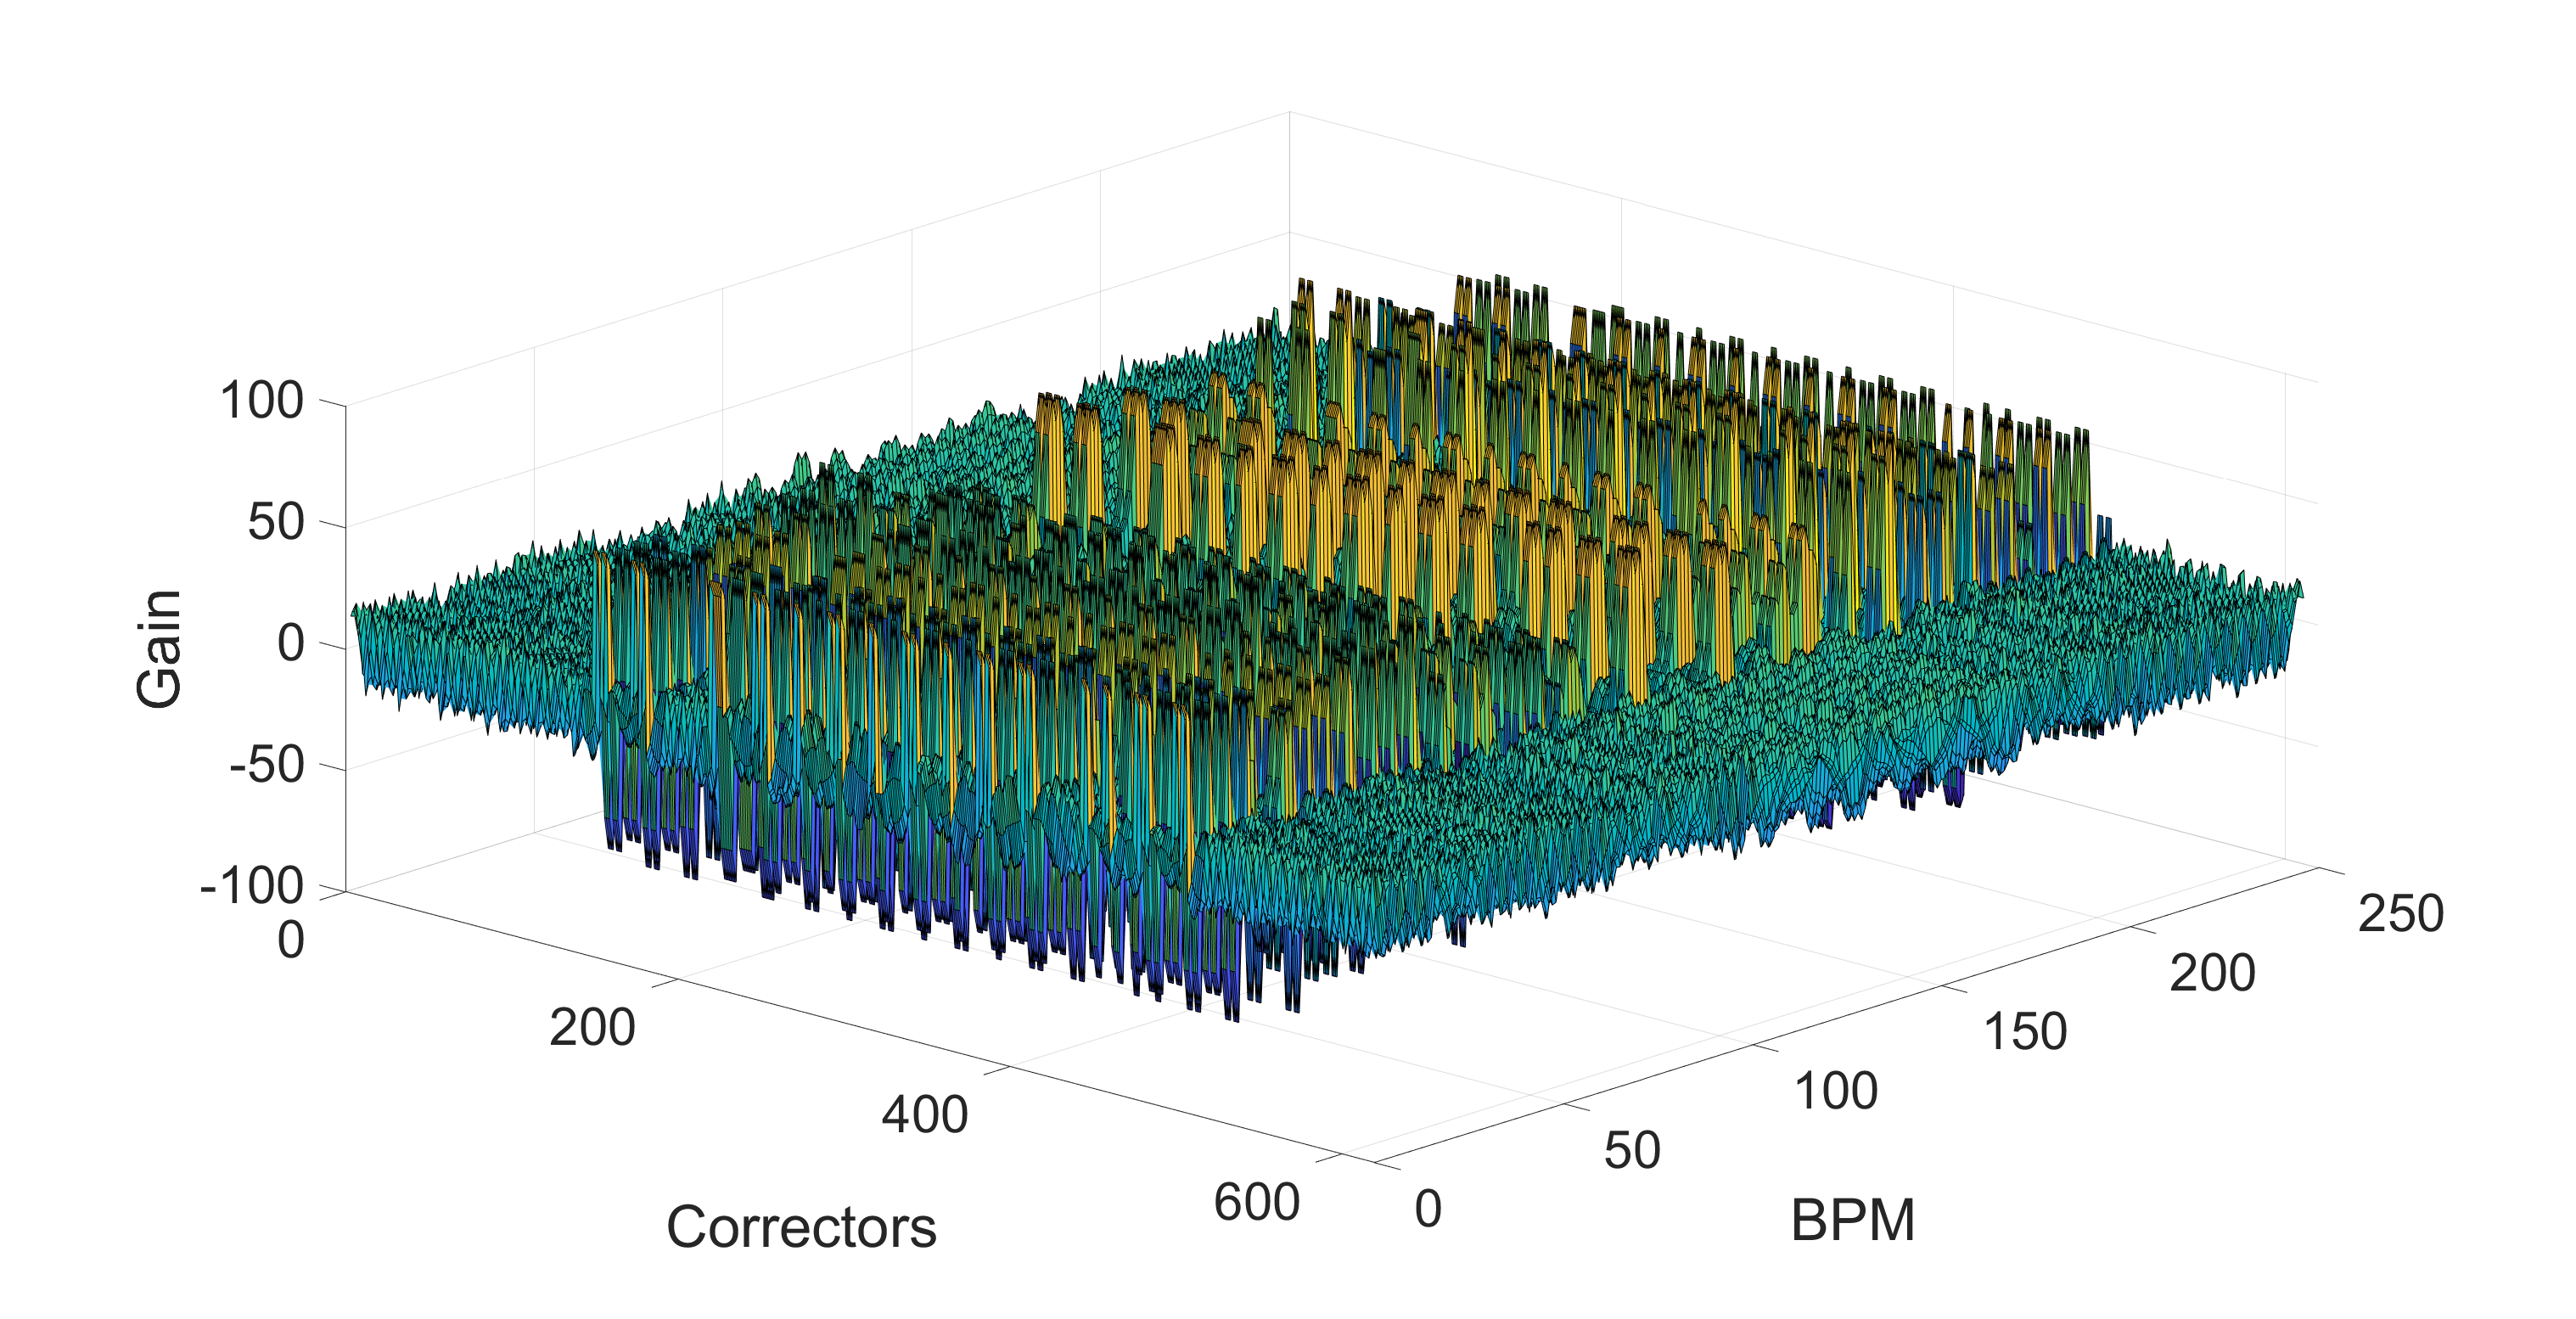
\includegraphics[scale=0.3]{R_y.eps}
    \end{center}
    \caption{Storage ring response matrix 3D plot (vertical).}
    \label{fig:R_y}
\end{figure}

\subsection{ORM inversion}

\subsection{Controller}

\subsubsection{Weighted SVD controller}

The controller is divided between the time-dependent filter and the part that depends only on the direction of the measurement vector $\vect{y}[k] + \vect{d}[k]$ (spatial filter). The objective of the spatial filter is to reconstruct the system states $\vect{x}[k]$ (correctors setpoints) from the data obtained by the BPM measurements $\vect{y}[k]$ and to suppress the noise at the same time. Without the noise, $\vect{x}[k]$ can be perfectly obtained by multiplying $\vect{y}[k]$ by the pseudo-inverse of the ring response vector $\matr{R}^{\dagger}$. However, the majority of synchrotron storage ring response matrices are ill-conditioned, this means that the condition number is very large. Practically, such a matrix is almost singular, and the computation of its inverse, or solution of a linear system of equations is prone to large numerical errors. A matrix that is not invertible has condition number equal to infinity \cite{leon2006linear}. 

The condition number is the ratio of the largest to the smallest singular value:
\begin{equation} \label{e:condition_number}
    \textrm{condition number} = \frac{s_1}{s_n} 
\end{equation}
\cite{pillow2018Statistical}.
To reduce the condition number of the pseudo-inverse of the response matrix $\matr{R}^{\dagger}$, the vector of measurements $\vect{y}[k]$ is multiplied by a modified matrix $\matr{\tilde{R}}^{\dagger}$ where the magnitudes of some of the singular values $s[i]$ have been reduced compared to $\matr{R}^{\dagger}$. To study which singular values $s[i]$ of $\matr{R}^{\dagger}$ have to be lowered, they are shown in figure \ref{fig:singular_values}. Most of the noise amplification occurs in the singular values with a high index $i$ and therefore a reduction of these values will result in less noise amplification.

\begin{figure}
    \begin{center}
        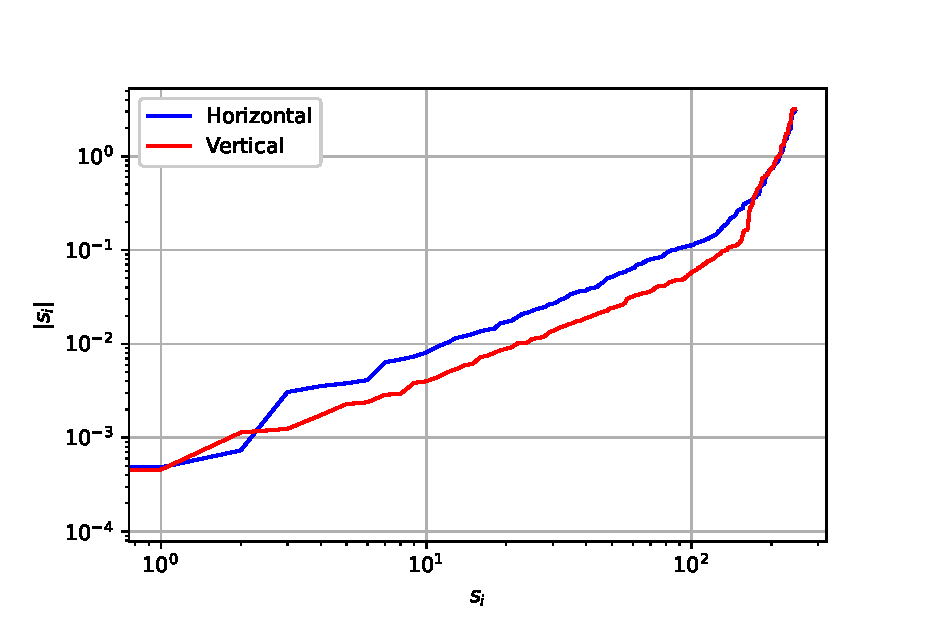
\includegraphics{singular_values.eps}
    \end{center}
    \caption{Magnitudes of the singular values $s[i]$ of the matrix $\matr{R}^{\dagger}$.}
    \label{fig:singular_values}
\end{figure}

Considering the facts that the first few $s[i]$ are able to mitigate the fluctuations in the beam and at the same time not amplify the noise too much, it is possible to create an efficient spatial filter. This is done by multiplying $\vect{y}[k]$ with $\matr{\tilde{R}}^{\dagger}=\matr{V}\matr{F}\matr{\Sigma}^{-1}\matr{U}^T$ where $\matr{F}$ is a diagonal matrix used to scale the singular values in $\matr{\Sigma}^{-1}$. In the case of the simulation of PETRA III the first 80 diagonal entries of of $\matr{F}$ are chosen to be 1, while all other entries are 0.

\subsubsection{Correction}


% \subsection{Electron Beam Stability}

% \subsection{Dynamical Process Model}

% \subsection{Spatial Process Model}

% \subsection{Control considerations}

% \subsection{Weighted SVD Controller}

% \subsection{Monitoring and Correction Instruments}

% \subsection{Orbit Correction Methods}

% \subsection{Correction}